\documentclass{article}
\usepackage[utf8]{inputenc}
\usepackage{float}
\usepackage{graphicx}

\title{Digital Methods: Learning Journal Template}
\author{Alexander Dueholm-Hansen}
\date{Autumn 2019}

\begin{document}

\maketitle

\section{First hands on lesson 2019/31/10 week 44}
\subsection{Thoughts / Intentions} I initially didn't know what i could use regular expressions for, but i found out in the end. 
\subsection{Action} We used a program which can find regular expressions in texts
\subsection{Results} we learned how to find dates and words and misspelled words
\subsection{Final Thoughts} this could be use full for a historian, for example if want to find specific words spelled differently you can use regular expressions. 

\pagebreak{}


\section{Regular Expressions 2019/04/11 week 45}
\subsection{Thoughts / Intentions} We have to recompile word lists for Voyant and R
\subsection{Action} I used the regular expressions program called Regex101.com. I first recompiled the word list for Voyant by finding the quotations and commas in the text and when using next line \textbackslash n in substitution, i when did it with R by first finding all newlines with command \textbackslash s and then substitute " and , and then ad " in the beginning and in the end. See pictures under results. You could also write (.+)\textbackslash n which finds all words and then write this "\$1", in the substitution which ads quotations and commas to all words.


\subsection{Results} See pictures with results next page
\begin{figure}[H]
    \centering
    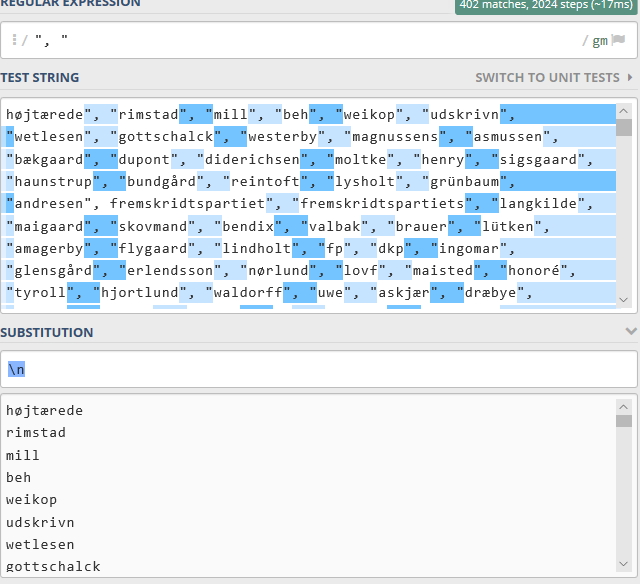
\includegraphics[width=\textwidth]{foto1.PNG}
    \caption{online regex100:}
    \label{fig:bil1}
\end{figure}
\begin{figure}[H]
    \centering
    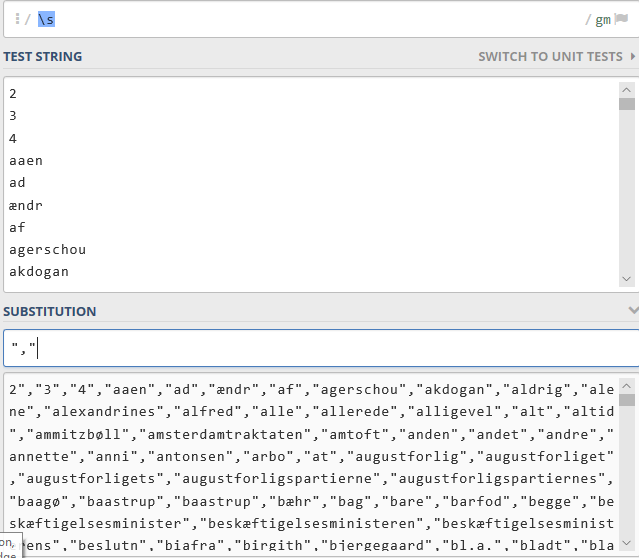
\includegraphics[width=\textwidth]{foto2.PNG}
    \caption{online regex100: You have to ad the quotation in the beginning and the end, which I forgot.}
    \label{fig:bil2}
\end{figure}
\begin{figure}[H]
    \centering
    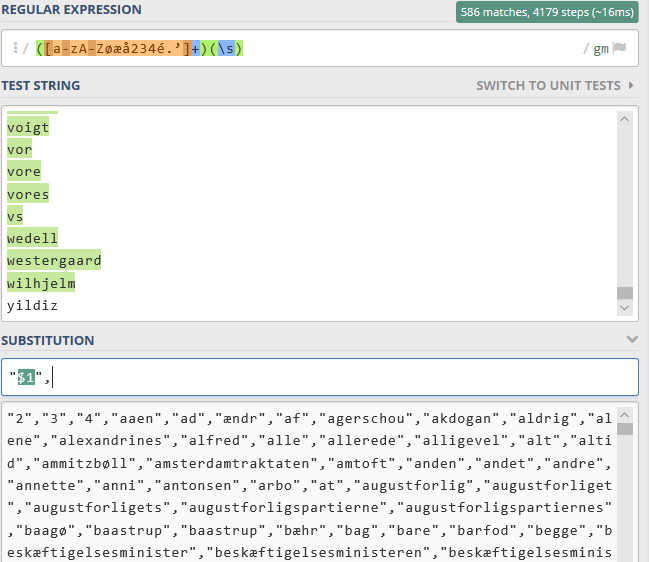
\includegraphics[width=\textwidth]{foto3.png}
    \caption{this is another "hard way" of doing it, where you get the quotations and commas in the right places the first time}
    \label{fig:bil3}
\end{figure}
\subsection{Final Thoughts} I had no idea what to do in the beginning but after reading the librarycarpenteri i slowly found out what to do.

\pagebreak{}

\section{Spreadsheets and datacleaning 2019/07/11 week 45}
\subsection{Thoughts / Intentions} We need to seperate dates, months and years in a date, and I initially thought why you should do it, and i could'nt find out how to do it?
\subsection{Action} After seen Adelas introduction on excel I found out. In excel i made three new columns and formated the cells to numbers with no decimals. I then named the first column day and wrote =dag() in the cell under and then pressed on the first date, and got the number 17 which I double clicked and got the rest of the days. I did the same process with months =måned() and years =år()
\subsection{Results}\
\begin{figure}[H]
    \centering
    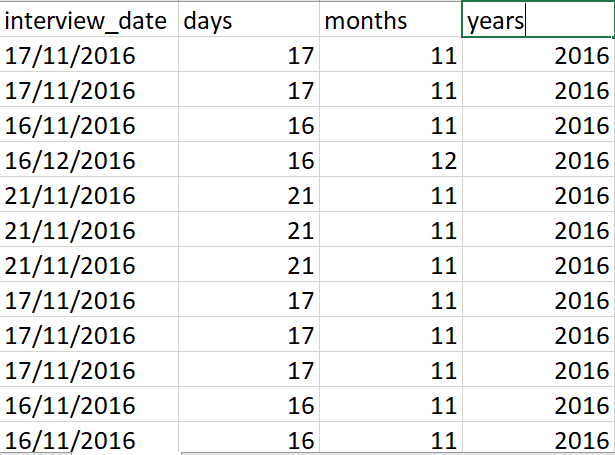
\includegraphics[width=\textwidth]{foto excel.PNG}
    \caption{excel}
    \label{fig:bil4}
\end{figure}
\subsection{Final Thoughts} I found out what you have to separate dates months and years because your dates wont change if you send them to americans or someone else with a different excel setup. \\\\

\section{Openrefine 2019/07/11 week 45}
\subsection{Thoughts / Intentions} First of all, I was a bit sceptical of what we could use openrefine for that excel could not do. 
\subsection{Action} We tried working with a messy ecxel dataset and cleaning it. 
\subsection{Results} We cleaned the dataset by choosing accepted values and recompiling values which sounded the same. 
\subsection{Final Thoughts} This program can do way more than Excel and I came to enjoy the program very much for example the search option.\\

\section{Openrefine 2019/28/11 week 45}
\subsection{Thoughts / Intentions} I will now show what you can use openrefine to do 
\subsection{Action} I will clean a csv.file from the Aarhus city councils https://raw.githubusercontent.com/aarhusstadsarkiv/datasets/master/minutes/city-council/city-council-minutes-1915-1930.csv I got it from aarhus city archives github and it is a url ending with csv. I open refine and choose the url option, and openrefine suggest that it is a csv file. Futher more it suggest seperating by commas. If we look in csv file we see this in the header. date\_of\_meeting,publication\_page,page\_url,record\_ids,text as we can see is it seperated by commas so click create project. We are only interested in the dates and text so we collapse the other columns. From here on we can start textmining and using facets, which I might do in my project.
\subsection{Results} 
\begin{figure}[H]
    \centering
    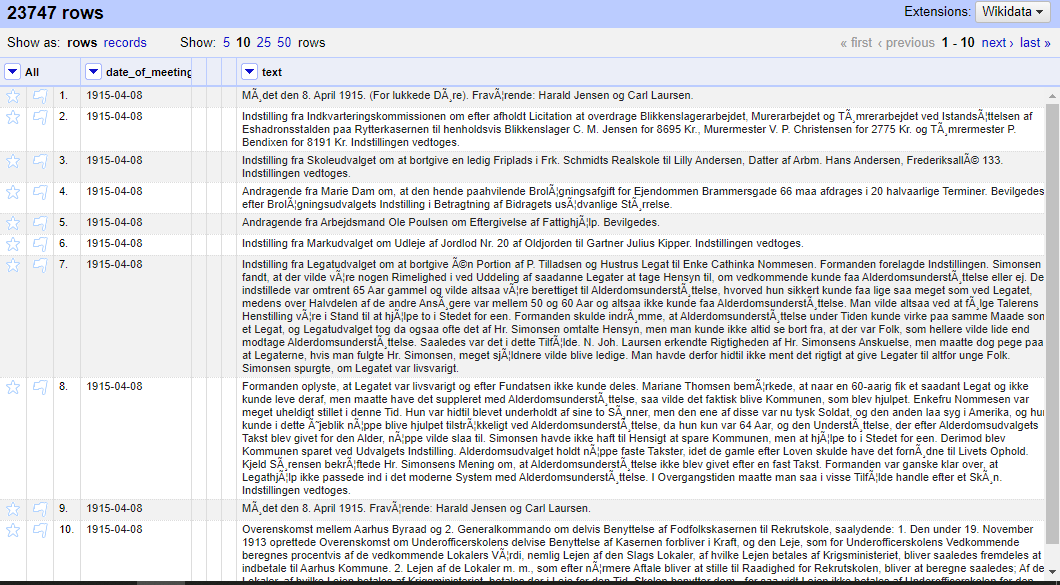
\includegraphics[width=\textwidth]{openrefine.PNG}
    \caption{excel}
    \label{fig:bil7}
\end{figure}\\

\subsection{Final Thoughts} The only problem is that there is a lot af text in the text column, so the facets are to big.\\\\

\section{Shell 2019/14/11 week 46}
\subsection{Thoughts / Intentions} I was really confused at first, is this just a difficult way of using pathfinder?  
\subsection{Action} We tried a lot of different commands, and got to learn the program, what backslash is, and how to navigate through folders
\subsection{Results} We learned how to create or own folders and text files in them. 
\subsection{Final Thoughts} at the end of the lesson you told us, that shell can handle more files that pathfinder and probably more, that we haven't learned yet. For example finding earlier versions of a file. \\\\

\section{R 2019/21/11 week 47}
\subsection{Thoughts / Intentions} I thought R would be a use full program, as we saw in the first lesson in this course with the UN votes.  
\subsection{Action} We got to know the program and how you write commands in the script 
\subsection{Results} we did some exercises, and learned what vectors can only be one datatype, and R will simply change the vectors to the same datatype. 
\subsection{Final Thoughts} This program has a lot of possibilities, which will be explored in upcoming tasks.  

\section{R task 2019/28/11 week 47}
\subsection{Thoughts / Intentions} In the introduction to R (https://datacarpentry.org/r-socialsci/01-intro-to-r/index.html) we had to do a lot of exercises. I have copied my notes from R into LaTex\\
\subsection{Action} exercise 1. First we had to change area(underscore)hectares to 2,5 which I did with this command area(underscore)hectares \textless- 2.5 and when i had to multiply with 2.47 and that i wrote like this area\_hectares \textless- 2.5 which is 6,175.\\\\

exercise 2. We had to create two variables length and width and assign them values. and thereafter create a third variable area and give it a value based on the current values of length and width. I have to show that changing the values of either length and width does not affect the value of area before I rerun the line. See results.\\\\

exercise 3. I had to type in ?round at the console and then look at the output in the Help pane. I saw that you can also use signif,  function that are similar to round? The digits parameter is used for diciding how many decimals see results exercise 3. \\\\

exercise 4. We have to see what happens when you mix vectors in these examples, see results for answers
num\_char \textless- c(1, 2, 3, "a")
 num\_logical \textless- c(1, 2, 3, TRUE)
 char\_logical \textless- c("a", "b", "c", TRUE)
 tricky \textless- c(1, 2, 3, "4")
 and combine them
 num\_logical \textless- c(1, 2, 3, TRUE)
char\_logical \textless- c("a", "b", "c", TRUE)
combined\_logical \textless- c(num\_logical, char\_logical)\\\\

Exercise 5. In this vector rooms \textless- c(1, 2, 1, 1, NA, 3, 1, 3, 2, 1, 1, 8, 3, 1, NA, 1) I have create a new vector with NA's removed from it by using this vector of rooms, create a new vector with the NAs removed, and thereafter the median of the rooms vector, and then find out how many houses have two rooms for sleeping. see results exercise 5.
exercise 6. in starting with data.
I first have to create a data frame (interviews\_100) containing only the data in row 100 of the interviews dataset.\\
I now have to use that number to pull out just that last row in the data frame and then compare that with what I saw as the last row by using tail() to make sure it’s meeting expectations. After that I have to pull out that last row using nrow() instead of the row number, and then create a new data frame (interviews(underscore)last) from that last row. Then I have to use nrow() to extract the row that is in the middle of the data frame and store the content of this row in an object named interview(underscore)middle.Last but not least I have to combine nrow() with the - notation above to reproduce the behavior of head(interviews), keeping just the first through 6th rows of the interviews dataset. See results exercise 6 for results\\\\

\subsection{Results} exercise 1. area\_hectares \textless- 2.5
\textgreater area(underscore)hectares*2.47
[1] 6.175\\\\

exercise 2. length \textless- 9
width \textless- 5
area \textless- length*width
area 45
length \textless- 10
width \textless- 5
area \textless- length*width
area [1] 45\\\\

exercise 3. ?round
round(3.14156, digits=2) round rounds up to nearest number, digits is how many decimals here 2. 
[1] 3.14
round(2,3.141456) you can't do this
round(digits=2,x=3.14156) this is another way of doing round(3.14156, digits=2) x is a function.\\\\

exercise 4. 
num\_char \textless- c(1, 2, 3, "a") all values gets quotations
 num\_logical \textless- c(1, 2, 3, TRUE) TRUE gets transformed to a 1
 char\_logical \textless- c("a", "b", "c", TRUE) TRUE gets quotations
 tricky \textless- c(1, 2, 3, "4") all values gets quotations
num\_logical \textless- c(1, 2, 3, TRUE)
char\_logical \textless- c("a", "b", "c", TRUE)
combined\_logical \textless- c(num(underscore)logical, char\_logical) only one true appears\\\\

Exercise 5. we need to find out how many houses with 2 rooms for sleeping. 
rooms \textless- c(1, 2, 1, 1, NA, 3, 1, 3, 2, 1, 1, 8, 3, 1, NA, 1)
rooms\_no\_na \textless- rooms[!is.na(rooms)] now we take away NA
median(rooms, na.rm = TRUE) thats calculates the median of the rooms vector.
[1] 1 which is 1
rooms\_above\_2 \textless- rooms\_no\_na[rooms\_no\_na \textgreater 2] now it finds all houses with 2 rooms 
length(rooms\_above\_2) how many houses with 2 rooms 
4 houses with 2 rooms for sleeping. \\


Exercise 6. 
\begin{figure}[H]
    \centering
    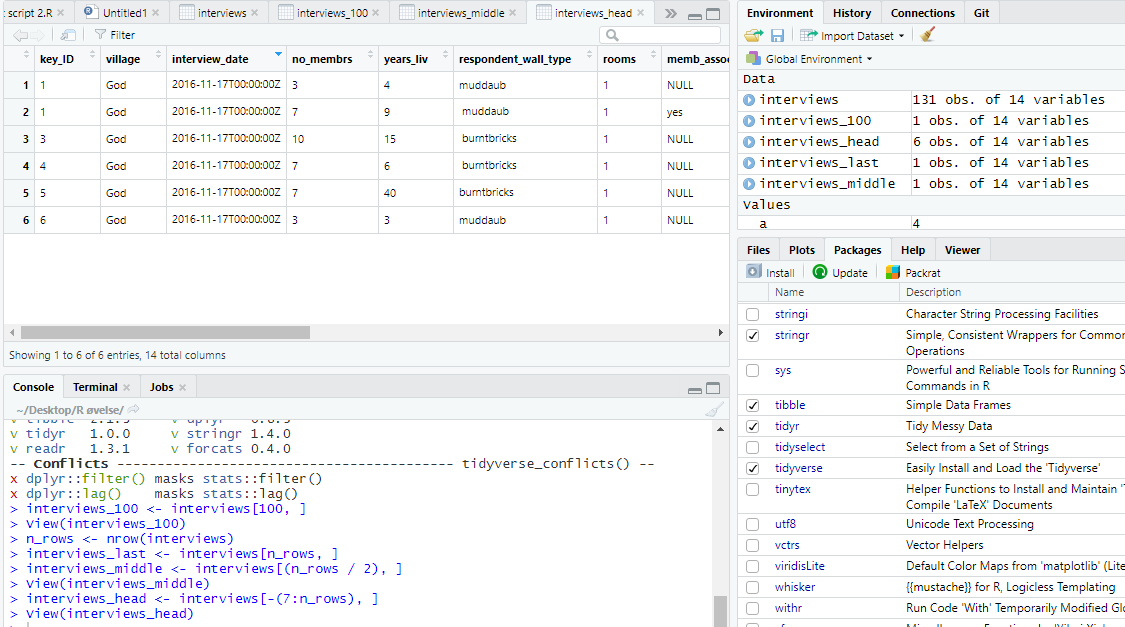
\includegraphics[width=\textwidth]{fotoR1.PNG}
    \caption{Rstudio}
    \label{fig:bil5}
\end{figure}

\subsection{Final Thoughts} The first tasks seemed like a difficult way of using a calculator but as I progressed in the tasks I found out that R can be used for so much more for example working with tables and illustrating them. 

\section{R tidyverse 2019/28/11 week 48}
\subsection{mixed notes and exercises from the day }   
tidyverse tools 28/11/2019 \\
library(tidyverse) we had to learn tidyverse which has a lot af diffent packages\\
interviews \textless- read\_csv("data/SAFI\_clean.csv", na="NULL")\\
view(interviews)\\\\

inspect my dataset\\
head(interviews)   Shows 6 first rows with 6 head columms\\
select(interviews, village, no\_membrs)   shows column village and no\_membrs \\\\

filter(interviews, village == "God")   all data only from the village God\\
  mutate () grows colums together. group\_by () is also functions like filter and select\\\\

Pipes\\
Interviews\_god \textless- interviews \%\textgreater\% can take the first product (God) and feeds into the next \\
  filter(village=="God") \%\textgreater\%\\
  select(village, no\_membrs)\\\\

interviews \%\textgreater\%\\
  mutate (people\_per\_room = no\_membrs/rooms)   we mutate the two colums\\\\

  na stands for not avalible, what we do doesn't effect the files before we save it. \\\\

interviews \%\textgreater\%\\
  filter (!is.na(memb\_assoc)) \%\textgreater\%   is is is not, and ! is a negation so we say don't include na\\
  mutate (people\_per\_room = no\_membrs/rooms)\\\\

 exercise 1 we have to find out how many total meals\\
interviews\_total\_meals \textless- interviews \%\textgreater\%   we create a new value from interviews called total meals\\
  mutate(total\_meals = no\_membrs * no\_meals) \%\textgreater\%   now we multiply members with meals and that is total\_meals \\
  filter(total\_meals \textgreater 20) \%\textgreater\%   now we filter all above 20\\
  select(village, total\_meals)   now we see all total meals above 20 because of the pipe\\
    we see now in the enviroment, the answer is 50\\\\

  analysis\\
interviews \%\textgreater\%\\
  group\_by(village) \%\textgreater\%   clustering rows of villages so we get 3 villages\\
  summarize(mean\_no\_membrs = mean(no\_membrs))   mean is average size of a family in the 3 villages \\\\

interviews \%\textgreater\%\\
  count(village)    how many responds from the villages \\

  exercise 2 we have to find out how many households in the survey have an average of two meals per day, Three meals per day, or other\\
interviews \%\textgreater\%\\
  count(no\_meals)   we do as above and see that there is 52 households with 2 meals and 79 with 3. \\
  now we have to use group\_by() and summarize() to find the mean, min, and max number of household members for each\\ village and also add the number of observations\\
interviews \%\textgreater\%\\
  group\_by(village) \%\textgreater\%   we group villages \\
  summarize(   and then summarize to find mean, min, max and n for number of observations\\
    mean\_no\_membrs = mean(no\_membrs),\\
    min\_no\_membrs = min(no\_membrs),\\
    max\_no\_membrs = max(no\_membrs),\\
    n = n()\\
  )\\
  this the result\\
  village  mean\_no\_membrs min\_no\_membrs max\_no\_membrs     n\\
  \textlesschr\textgreater             \textlessdbl\textgreater         \textlessdbl\textgreater         \textlessdbl\textgreater \textlessint\textgreater\\
  1 Chirodzo           7.08             2            12    39\\
  2 God                6.86             3            15    43\\
  3 Ruaca              7.57             2            19    49\\
  we see the mean, min and max for every village and total observations \\\\

  we need to find out what the largest household interviewed in each month was. \\

library(lubridate)   we use this package, and finds the day, months and years from the intervievdate\\
interviews \%\textgreater\%\\
  mutate(month = month(interview\_date), \\
         day = day(interview\_date),\\
         year = year(interview\_date)) \%\textgreater\%\\
  group\_by(year, month) \%\textgreater\%\\
  summarize(max\_no\_membrs = max(no\_membrs))\\
  results \\
  A tibble: 5 x 3\\
  Groups:   year [2]\\
  year month max\_no\_membrs\\
 \textlessdbl\textgreater \textlessdbl\textgreater         \textlessdbl\textgreater\\
  1  2016    11            19\\
  2  2016    12            12\\
  3  2017     4            17\\
  4  2017     5            15\\
  5  2017     6            15\\
  we see now how many household members in the biggest each month. \\\\

  exercise 3\\
  we have to Create a new data frame (named interviews\_months\_lack\_food) that has one column for each month and records TRUE or FALSE for whether each interview respondent was lacking food in that month.\\
interviews\_months\_lack\_food \textless- interviews \%\textgreater\%   we create a new dataframe called months lack food\\
  separate\_rows(months\_lack\_food, sep=";") \%\textgreater\%   we look at september\\
  mutate(months\_lack\_food\_logical  = TRUE) \%\textgreater\%   we put together dataframe with logical\\
  spread(key = months\_lack\_food, value = months\_lack\_food\_logical, fill = FALSE)   we record true and false\\
  we find out by looking in the dataframe hows many lacks food in sep.\\
  We see how many months (on average) were respondents without food if they did belong to an irrigation association.\\
interviews\_months\_lack\_food \%\textgreater\%\\
  mutate(number\_months = rowSums(select(., Apr:Sept))) \%\textgreater\%   we choose all months april to sep and mutate each month\\
  group\_by(memb\_assoc) \%\textgreater\%   we group members\\
  summarize(mean\_months = mean(number\_months))   we summarize the mean\\
  and finds A tibble: 3 x 2\\
  memb\_assoc mean\_months\\
  \textlesschr\textgreater            \textlessdbl\textgreater\\
   1 no                2.31\\
  2 yes               2.64\\
  3 NA                2.95\\
  2,6 months people with waterirrigation was without food and so on. \\\\

  plotting\\
interviews\_plotting \textless- interviews \%\textgreater\%\\
     spread data by items\_owned\\
  separate\_rows(items\_owned, sep=";") \%\textgreater\%\\
  mutate(items\_owned\_logical = TRUE) \%\textgreater\%\\
  spread(key = items\_owned, value = items\_owned\_logical, fill = FALSE) \%\textgreater\%\\
  rename(no\_listed\_items = `\textlessNA\textgreater`) \%\textgreater\%\\
     spread data by months\_lack\_food\\
  separate\_rows(months\_lack\_food, sep=";") \%\textgreater\%\\
  mutate(months\_lack\_food\_logical = TRUE) \%\textgreater\%\\
  spread(key = months\_lack\_food, value = months\_lack\_food\_logical, fill = FALSE) \%\textgreater\%\\
     add some summary columns\\
  mutate(number\_months\_lack\_food = rowSums(select(., Apr:Sept))) \%\textgreater\%\\
  mutate(number\_items = rowSums(select(., bicycle:television)))\\\\

interviews\_plotting\\\\

write\_csv(interviews\_plotting, path = "output\_data/interviews\_plotting.csv")\\\\

  ggplot(data = \textlessDATA\textgreater, mapping = aes(\textlessMAPPINGS\textgreater)) +  \textlessGEOM\_FUNCTION\textgreater() \\
  ggplot tell which data, the athestics og how it is supposed to be function\\\\

ggplot(data = interviews\_plotting, aes(x = no\_membrs, y = number\_items)) + geom\_line ()\\\\

my\_plot \textless- ggplot(data = interviews\_plotting, aes(x = no\_membrs, y = number\_items))\\\\

my\_plot +\\
  geom\_line(color = "orange")   we change the color of the line\\\\

my\_plot +\\
  geom\_jitter(color="black", alpha = 0.5)   we change the color of the dots\\
\begin{figure}[H]
    \centering
    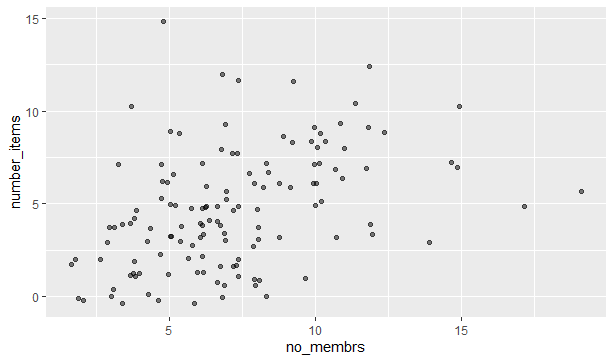
\includegraphics[width=\textwidth]{Rplot.png}
    \caption{Rstudio:}
    \label{fig:bil10}  
\end{figure}

ggplot(data = interviews\_plotting, aes(x = no\_membrs, y = number\_items)) +\\
  geom\_jitter(aes(color = village), alpha = 0.5)   we give each village a color\\

 exercise 4 create a scatter plot of rooms by village with the respondent\_wall\_type showing in different colors\\
ggplot(data = interviews\_plotting, aes(x = village, y = rooms)) +   we have villages horizontial and rooms vertical\\
  geom\_jitter(aes(color = respondent\_wall\_type))   we give each walltype a color\\
  it is difficult to see each village\\

  boxplots
ggplot(data = interviews\_plotting, aes(x = respondent\_wall\_type, y = rooms)) +\\
  geom\_boxplot()   we create boxplots with the walltypes horisontial and rooms vertical\\
  If we ad points to the boxplot, we can have a better idea of the number of measurements and of their distribution:\\
  
  ggplot(data = interviews\_plotting, aes(x = respondent\_wall\_type, y = rooms)) + \\
  geom\_boxplot(alpha = 0) +   we make a boxplot\\
  geom\_jitter(alpha = 0.5, color = "tomato")   we give the points color\\

\begin{figure}[H]
    \centering
    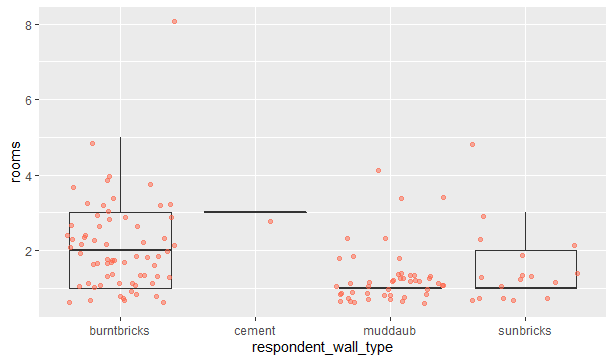
\includegraphics[width=\textwidth]{boxplot.png}
    \caption{Rstudio:}
    \label{fig:bil10}  
\end{figure}

  exercise 5. we need to replace the box plot with a violin plot\\
  ggplot(data = interviews\_plotting, aes(x = respondent\_wall\_type, y = rooms)) +\\
    geom\_violin(alpha = 0) +   we do that by changing it from boxplot to violin\\
    geom\_jitter(alpha = 0.5, color = "tomato")\\

\begin{figure}[H]
    \centering
    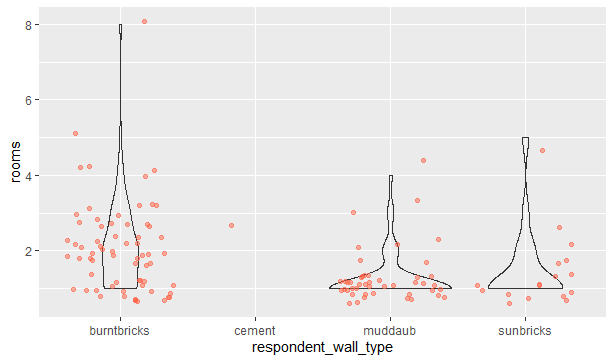
\includegraphics[width=\textwidth]{violin.png}
    \caption{Rstudio:}
    \label{fig:bil11}  
\end{figure}
  
  we now have to make a new plot to explore the distribution of another variable within wall type.\\
  We have to create a boxplot for liv\_count for each wall type and then overlay the boxplot layer on a jitter layer to show actual measurements.\\
  ggplot(data = interviews\_plotting, aes(x = respondent\_wall\_type, y = liv\_count)) +\\
    geom\_boxplot(alpha = 0) +\\
    geom\_jitter(alpha = 0.5)\\
  and then add color to the data points on the boxplot according to whether the respondent is a member of an irrigation association\\
  ggplot(data = interviews\_plotting, aes(x = respondent\_wall\_type, y = liv\_count)) +\\
    geom\_boxplot(alpha = 0) +\\
    geom\_jitter(aes(alpha = 0.5, color = memb\_assoc))\\

\begin{figure}[H]
    \centering
    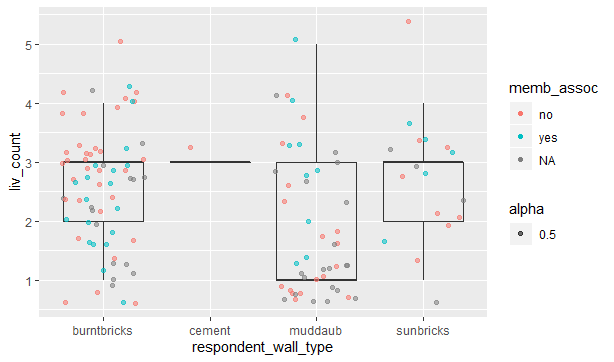
\includegraphics[width=\textwidth]{bloxplot 5.png}
    \caption{Rstudio:}
    \label{fig:bil12}  
\end{figure}

\end{document}
